\balancecolumns\newpage\ \\\newpage
\appendix
\section{Source Code Structure}


The source code for the ESP framework is organized as follows.

\begin{itemize}

\item \textbf{Registry}

The code for the registry is under the "registry" directory.  config.py contains information regarding the SQL database connection attributes including the username, password, and database
name.  difdbi.py contains helper functions to add various components of a ESPml document to the database.  registry.py contains the SOAP server implementation that has all the interfaces
defined and then calls the appropriate functions to interact with the database.  registry\_client.py is a sample client that can test the registry.

\item \textbf{XML}

All the XML files associated with the ESP framework is stored in the XML directory.  espml.py, espmlsubs.py, and query.py are XML parsing utilities that help in representing a ESPml
document in terms of python objects.  The actual schema is named espml.xsd and an example system is named system1.xml.  Examples of ESPml queries and responses are presented as
locationQuery.xml and query\_response.xml. 

\item \textbf{Web Client}

The files that represent the geo-centric client are in the web directory.  index.html contains all the Java Script code to represent the Google Map and also interact with the map.  createHTML.py
actually makes queries and gets the response to them which the Java Script can use to display on the Google Map.  callFunction.py is a SOAP client that actually makes the web services calls to 
a system.  baseFunctionCall.xml is a template used to make function calls.

\item \textbf{System}

The files representing the base system and all the example network systems designed for this project are in the system directory.  system.py is a template for a typical network system. 
The rest of the files associated with each unique network system are under their corresponding directory name.  These include such things as sonycam, iTunes, beachCams, weather, and sos.

\end{itemize}

\begin{figure}[b]
  \begin{center}
  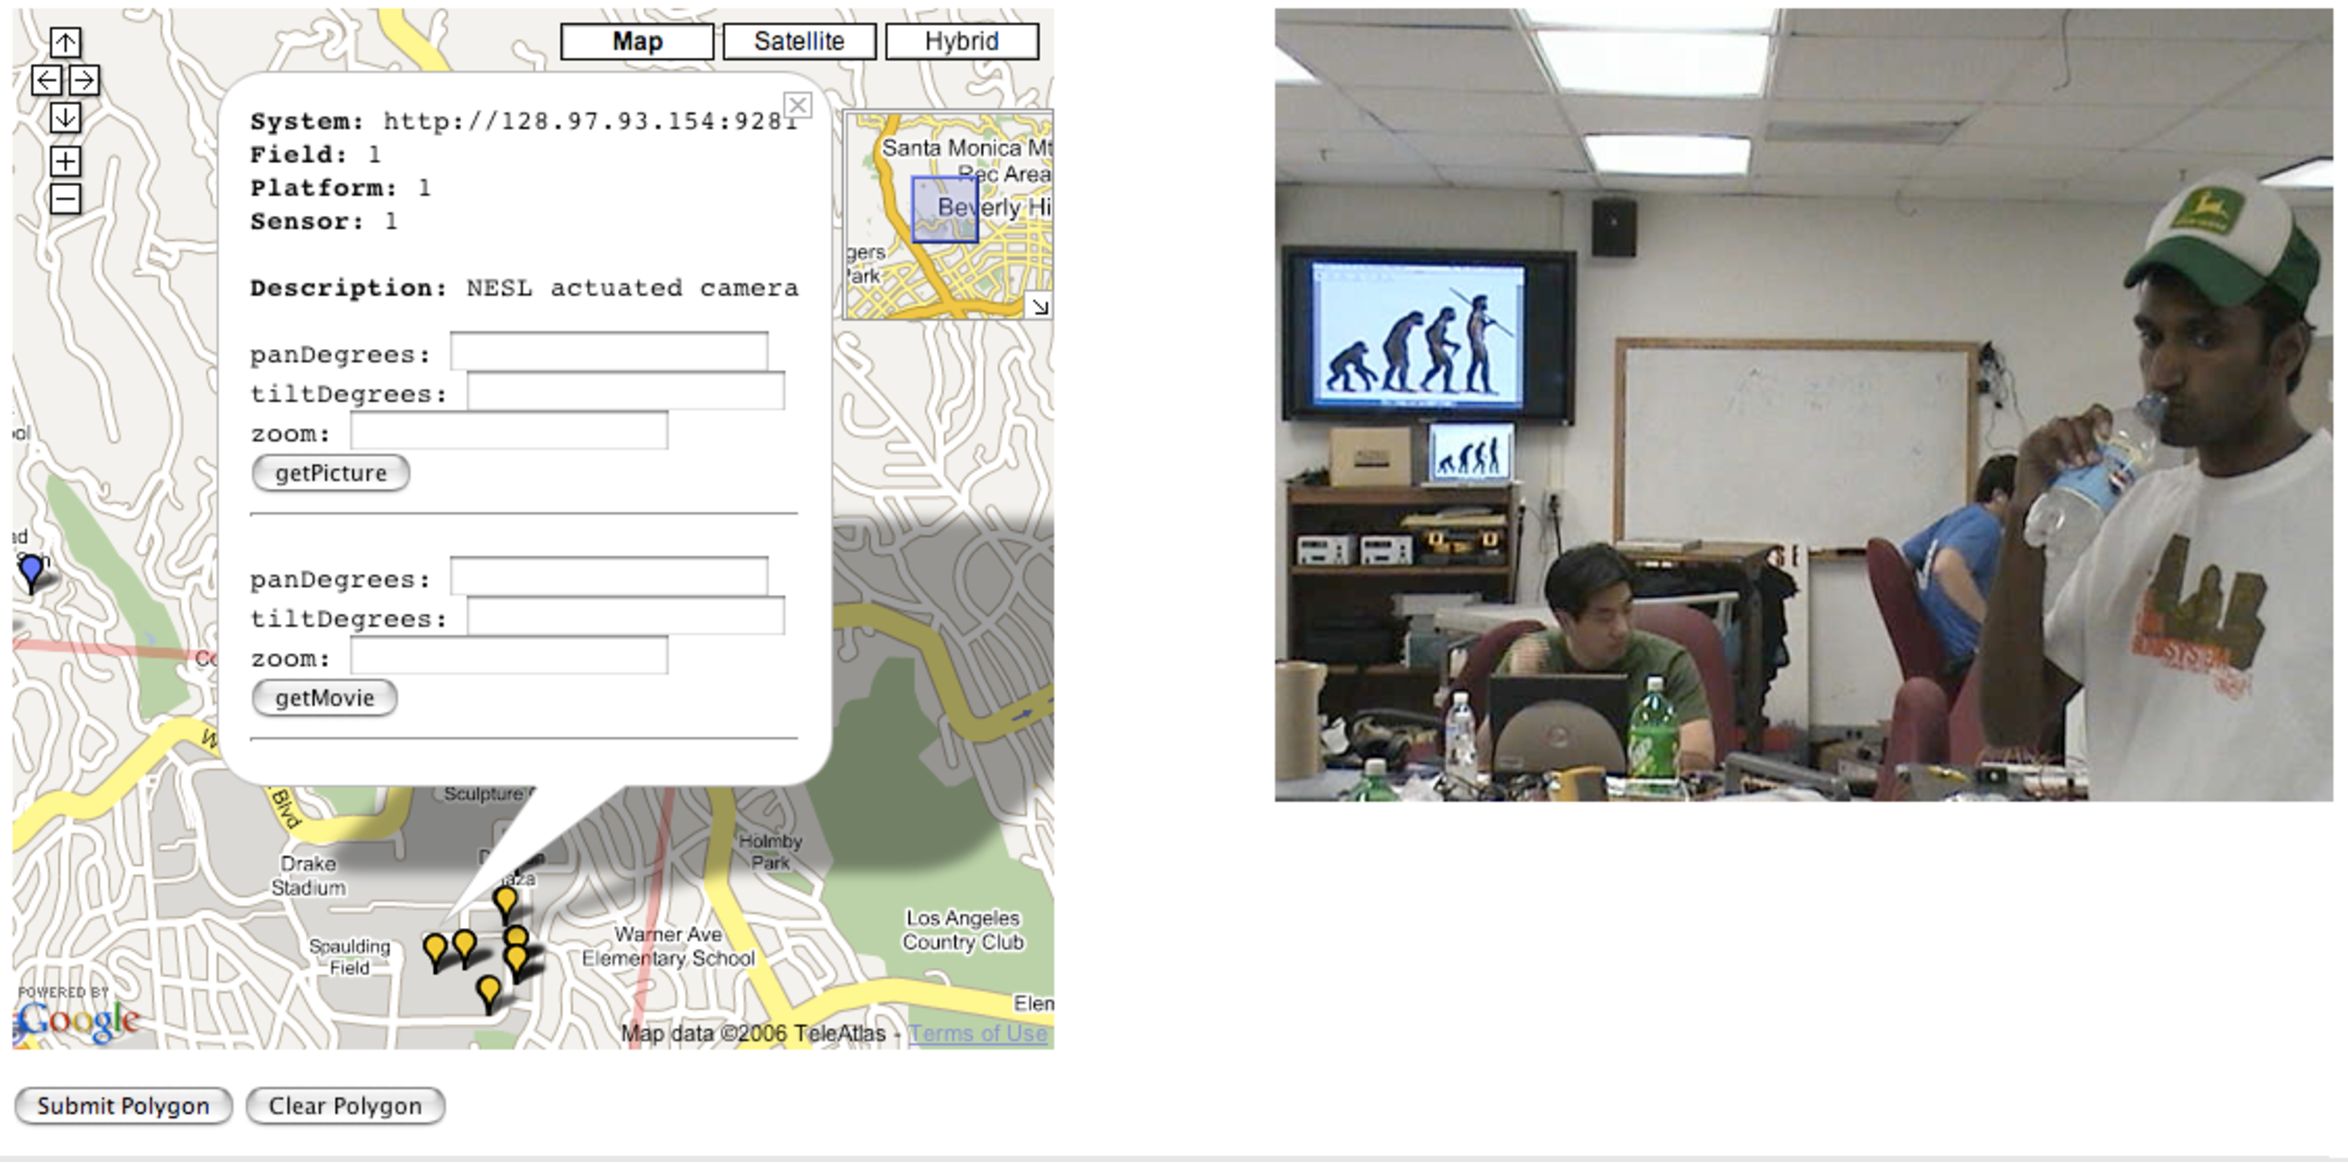
\includegraphics[width=0.49\textwidth]{images/ui1}
  \caption{Screen-shot of the Google Maps client and an actuated camera.}
  \label{fig:ui1}
  \end{center}
\end{figure}

\begin{figure}[h]
  \begin{center}
  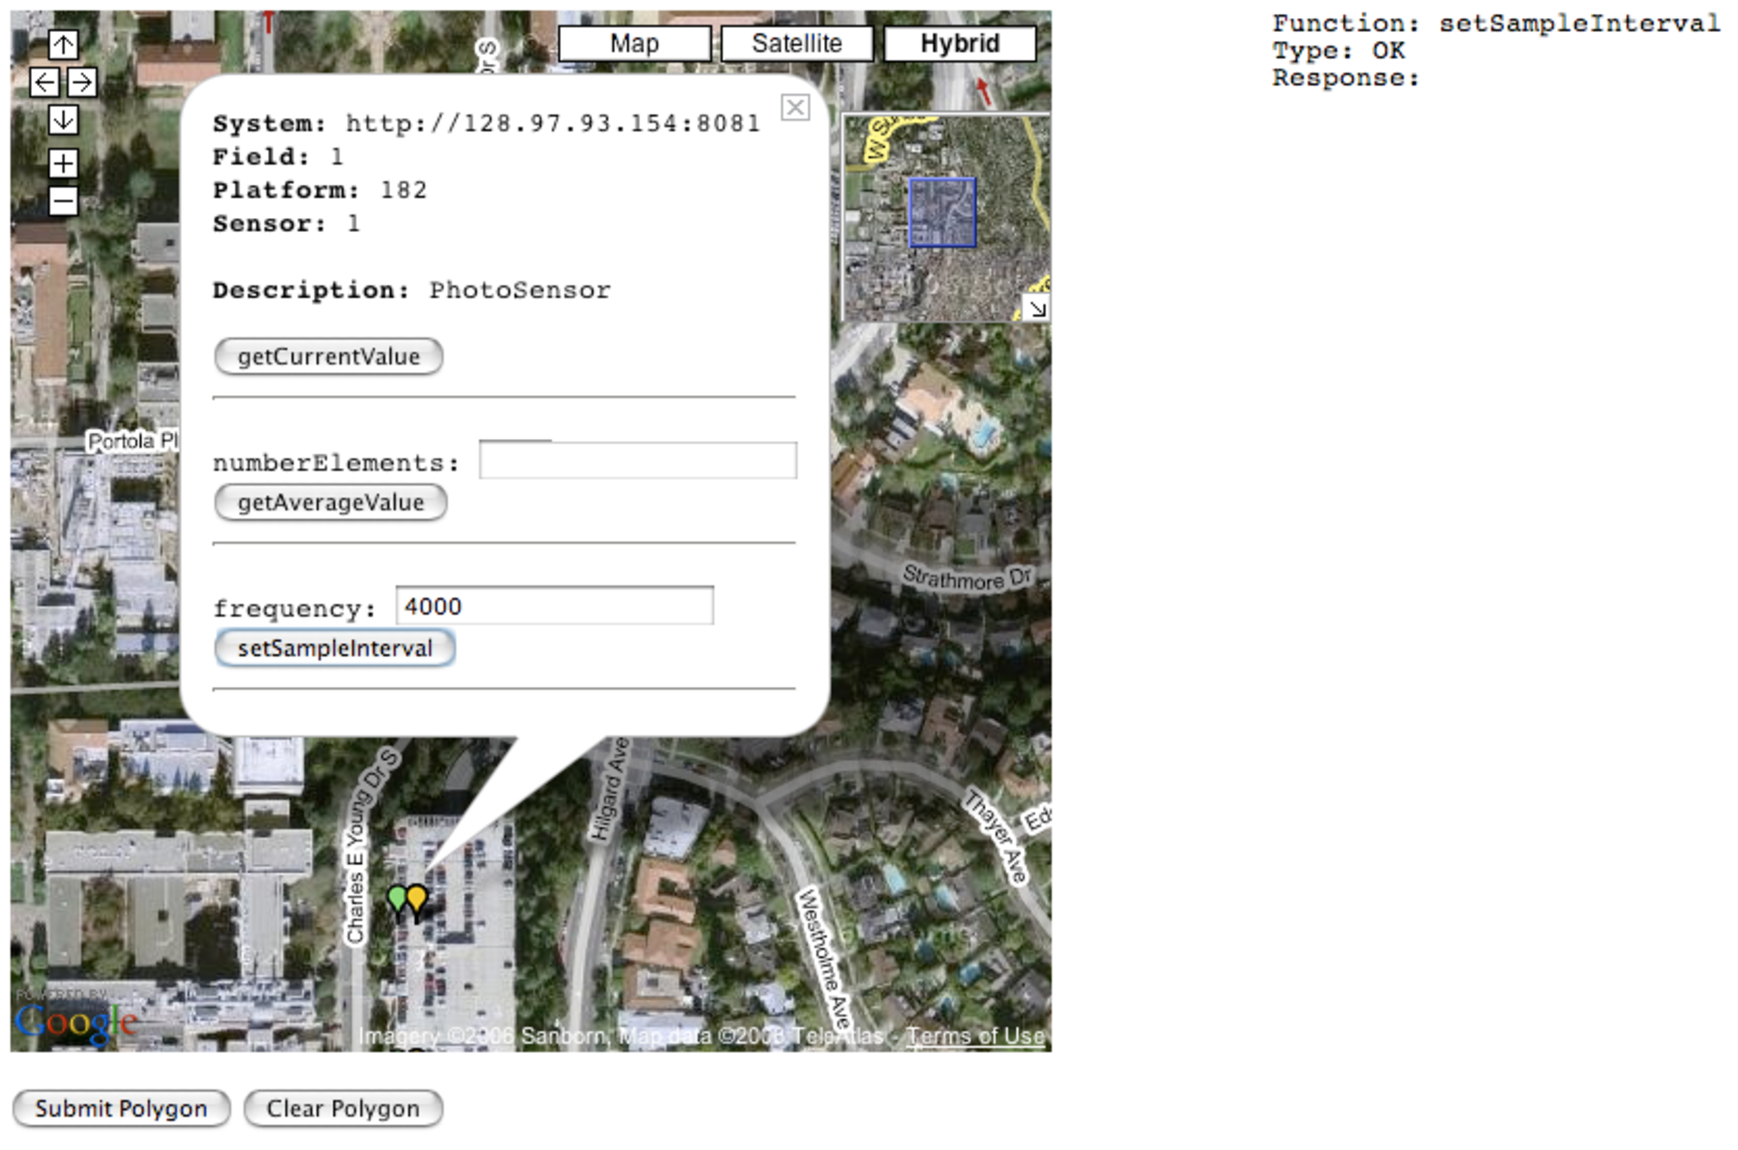
\includegraphics[width=0.45\textwidth]{images/ui2}
  \caption{Screen-shot of the Google Maps client and a small sensor
  network node's photodiode sensor.}
  \label{fig:ui2}
  \end{center}
\end{figure}

\begin{figure}[b!]
  \begin{center}
  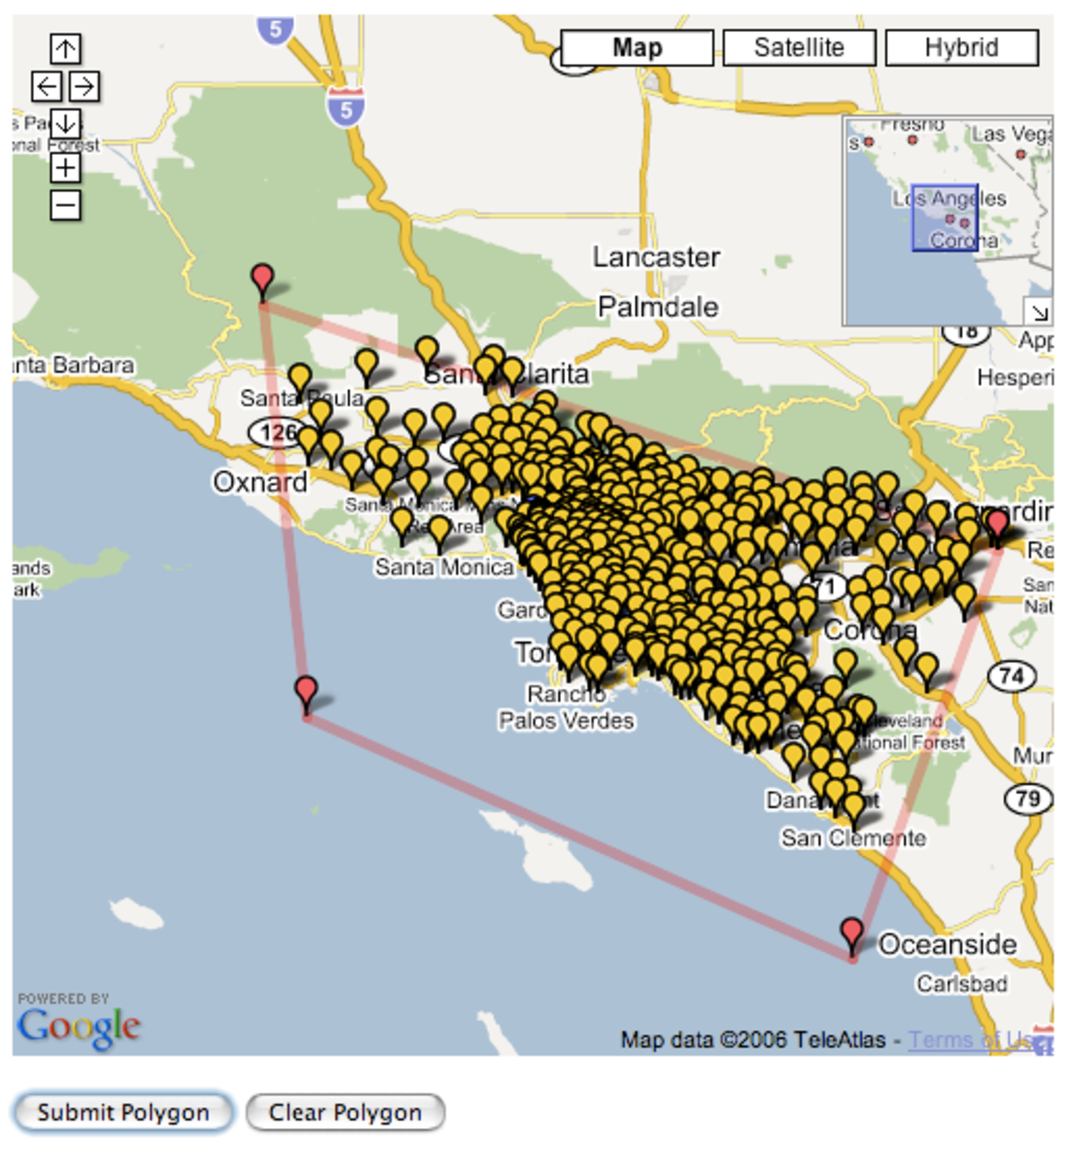
\includegraphics[width=0.35\textwidth]{images/ui3}
  \caption{Screen-shot of the Google Maps client and the weather
  stations in the Los Angeles area.}
  \label{fig:ui3}
  \end{center}
\end{figure}

\section{UI Examples}
Figures \ref{fig:ui1}, \ref{fig:ui2}, and \ref{fig:ui3} depict screen-shots of the
Google Maps client interface.



\section{ESPml Schema}
Figure \ref{fig:espml_schema} shows the ESPml schema as of writing
this report. Note that the schema is under development and might have
changed. Please contact the authors if you are interested in
the latest version.

\begin{figure*}[h]
\lstset{basicstyle=\tiny,breaklines=true}
\begin{lstlisting}
<?xml version="1.0" encoding="UTF-8"?>
<xs:schema xmlns:xs="http://www.w3.org/2001/XMLSchema">
    <xs:element name="system">
        <xs:complexType>
            <xs:sequence>
                <xs:element name="id" type="xs:anyURI"/>
                <xs:element name="field" minOccurs="1" maxOccurs="unbounded">
                    <xs:complexType>
                        <xs:sequence>
                            <xs:element ref="id"></xs:element>
                            <xs:element ref="location"></xs:element>
                            <xs:element ref="description"></xs:element>
                            <xs:element ref="function" minOccurs="0" maxOccurs="unbounded"></xs:element>
                            <xs:element name="platform" minOccurs="1" maxOccurs="unbounded">
                                <xs:complexType>
                                    <xs:sequence>
                                        <xs:element ref="id"></xs:element>
                                        <xs:element ref="location"></xs:element>
                                        <xs:element ref="description"></xs:element>
                                        <xs:element ref="function" minOccurs="0"
                                            maxOccurs="unbounded"/>
                                        <xs:element name="sensor" minOccurs="0" maxOccurs="unbounded">
                                            <xs:complexType>
                                                <xs:sequence>
                                                  <xs:element ref="id"></xs:element>
                                                  <xs:element ref="location"></xs:element>
                                                  <xs:element ref="description"/>
                                                  <xs:element ref="function" minOccurs="0" maxOccurs="unbounded"/>
                                                  <xs:element name="type" type="xs:string"/>
                                                </xs:sequence>
                                            </xs:complexType>
                                        </xs:element>
                                    </xs:sequence>
                                </xs:complexType>
                            </xs:element>
                        </xs:sequence>
                    </xs:complexType>
                </xs:element>
            </xs:sequence>
        </xs:complexType>
    </xs:element>
    <!-- Simple element definitions -->
    <xs:element name="id" type="xs:integer"/>
    <xs:element name="description" type="xs:string"/>

    <!-- Complex element definitions -->
    <xs:element name="function">
        <xs:complexType>
            <xs:sequence>
                <xs:element name="description" type="xs:string"></xs:element>
                <xs:element name="parameter" minOccurs="0" maxOccurs="unbounded">
                    <xs:complexType>
                        <xs:sequence>
                            <xs:element name="description" type="xs:string"></xs:element>
                            <xs:element name="value" minOccurs="0" maxOccurs="1" type="xs:string"></xs:element>
                        </xs:sequence>
                        <xs:attribute name="name" type="xs:string"/>
                    </xs:complexType>
                </xs:element>
                <xs:element name="output" minOccurs="0" maxOccurs="unbounded">
                    <xs:complexType>
                        <xs:sequence>
                            <xs:element name="URI" minOccurs="1" maxOccurs="1" type="xs:anyURI"></xs:element>
                        </xs:sequence>
                        <xs:attribute name="type" type="xs:string"/>
                    </xs:complexType>
                </xs:element>
            </xs:sequence>
            <xs:attribute name="name" type="xs:string"/>
        </xs:complexType>
    </xs:element>

    <xs:element name="location">
        <xs:annotation>
            <xs:documentation>Point: Specify three values representing x,y,z coordintes.</xs:documentation>
            <xs:documentation>Polygon:  Must be four pairs of x,y,z coordinates with last being identical to the first..</xs:documentation>
        </xs:annotation>
        <xs:complexType>
            <xs:sequence>
                <xs:element name="Mobile" minOccurs="0" maxOccurs="1"></xs:element>
                <xs:choice>
                    <xs:element name="point" minOccurs="1" maxOccurs="unbounded">
                        <xs:complexType>
                            <xs:sequence>
                                <xs:element name="pos" type="xs:string"/>
                            </xs:sequence>
                        </xs:complexType>
                    </xs:element>
                    <xs:element name="polygon" minOccurs="1" maxOccurs="unbounded">
                        <xs:complexType>
                            <xs:sequence>
                                <xs:element name="poslist" type="xs:string"/>
                            </xs:sequence>
                        </xs:complexType>
                    </xs:element>
                </xs:choice>
            </xs:sequence>
        </xs:complexType>
    </xs:element>
    <xs:element name="query">
        <xs:complexType>
            <xs:sequence>
                <xs:element ref="system" minOccurs="1" maxOccurs="unbounded"></xs:element>
            </xs:sequence>
        </xs:complexType>
    </xs:element>
</xs:schema>

\end{lstlisting}
\caption{ESPml schema used in the framework.}
\label{fig:espml_schema}
\end{figure*}


\section{ESPml Examples}
Figure \ref{fig:espml_example} shows an example for an ESPml document
which would be sent to the registry. It consists of three platforms
with id's 1, 182, and 196. Platform 1 has no sensors nor
functions. Platform 182 and 196 are equivalent and have one
photosensor connected. There are definitions for functions which act
on the field, or on the individual sensors themselves.

\begin{figure*}
\lstset{basicstyle=\tiny,breaklines=true}
\begin{lstlisting}
<?xml version="1.0" encoding="UTF-8"?>
<system xmlns:xsi="http://www.w3.org/2001/XMLSchema-instance"
 xsi:noNamespaceSchemaLocation="../../xml/espml.xsd">
 <id>http://foobar.com:8081</id>
 <field>
  <id>1</id>
  <location>
   <polygon>
    <poslist>34.0815,-118.46,0.00 34.0518,-118.46,0.00 34.0509,-118.42,0.00 34.0805,-118.42,0.00
     34.0815,- 18.46,0.00</poslist>
   </polygon>
  </location>
  <description>This is a small test field of SOS nodes.</description>
  <function name="getCurrent">
   <description>Returns the current values for all platforms in this field.</description>
  </function>
  <function name="average">
   <description>Returns the average over all platforms in this field. </description>
  </function>

  <platform>
   <id>1</id>
   <location>
    <point>
     <pos>34.0689,-118.44,0.00</pos>
    </point>
   </location>
   <description>MicaZ Basestation connected to the gateway.</description>
  </platform>

  <platform>
   <id>182</id>
   <location>
    <point>
     <pos>34.0689,-118.44,0.00</pos>
    </point>
   </location>
   <description>MicaZ node with Mica Sensor Board.</description>
   <sensor>
    <id>1</id>
    <location>
     <point>
      <pos>34.0689,-118.44,0.00</pos>
     </point>
    </location>
    <description>PhotoSensor</description>
    <function name="getCurrentValue">
     <description>Get's the current value for this sensor. </description>
    </function>
    <function name="getAverageValue">
     <description>Gets the average for this sensor. </description>
     <parameter name="numberElements">
      <description>The number of elements for which the average should be calculated. </description>
     </parameter>
    </function>
    <function name="setSampleInterval">
     <description>Sets the sampling frequency for this sensor. </description>
     <parameter name="frequency">
      <description>The frequency at which the sensor should sample. </description>
     </parameter>
    </function>
    <type>Light</type>
   </sensor>
  </platform>

  <platform>
   <id>196</id>
   <location>
    <point>
     <pos>34.0682,-118.44,0.00</pos>
    </point>
   </location>
   <description>MicaZ node with Mica Sensor Board.</description>
   <sensor>
    <id>1</id>
    <location>
     <point>
      <pos>34.0682,-118.44,0.00</pos>
     </point>
    </location>
    <description>PhotoSensor</description>
    <function name="getCurrentValue">
     <description>Get's the current value for this sensor. </description>
    </function>
    <function name="getAverageValue">
     <description>Gets the average for this sensor. </description>
     <parameter name="numberElements">
      <description>The number of elements for which the average should be calculated. </description>
     </parameter>
    </function>
    <function name="setSampleInterval">
     <description>Sets the sampling frequency for this sensor. </description>
     <parameter name="frequency">
      <description>The frequency at which the sensor should sample. </description>
     </parameter>
    </function>
    <type>Light</type>
   </sensor>
  </platform>

 </field>
</system>
\end{lstlisting}
\caption{Example for an ESPml XML document which would be sent to the
registry.}
\label{fig:espml_example}
\end{figure*}



